\chapter{Experiment Setup}

In this chapter, we present approaches for attacking machine learning algorithms with adversarial techniques presented in the previous chapter. We discuss that the knowledge of the architecture and weight parameters is sufficient to derive adversarial samples against DNNs. Further discussion goes into black box attacks where the attack has minimal information about the underlying system. The discussion is then closed with how model's knowledge can be transferred between different algorithms/techniques.
\section{CIFAR and ImageNet Datasets}

Improvements on Computer Vision were possible due to two main reasons: increased computational power and standardized datasets for benchmarking. The ever increasing amount of image data on the Internet fostered more sophisticated and robust algorithms to work on images and multimedia data. ImageNet is a large-scale ontology of images with 1.000 different classes and with 3.2 million 224x224 high resolution images in total \cite{deng2009imagenet}. CIFAR, on the other hand, is a more compact dataset with 32x32 colour images in 10 or 100 classes. The dataset consists of 60.000 images with equal amount of samples per class \cite{krizhevsky_2009}.

Even though both datasets differ on image sizes and number of class labels, they have similar data domain. CIFAR can be seen as a subset of ImageNet dataset, therefore, convolutional filters from the latter could be used to improve performance of the former as shown by Yosinski et al.(2014). 

Our experiment uses an imbalanced CIFAR10 on a VGG16 architecture initialized with ImageNet weights. This drastically improves the accuracy of the model when compared to one that was only trained on the CIFAR dataset. Having a better overall accuracy implies into a better feature space exploration, and, therefore a more robust model. The main reason for this approach is that we want to test adversarial robustness on models that perform similarly to current state of the art deep learning systems.

\section{The VGG Architecture}

As described on Chapter 2, a ConvNet is a sequence of layers, and every layer transforms one volume of activations to another through a differentiable function. Three main types of layers are used to build these networks: Convolutional Layer, Pooling Layer and Fully-Connected Layer.A Convolutional Layer would compute the output of neurons that are connected to local regions in the input, an Activation layer (RELU, Sigmoid etc) will apply elementwise functions, the Pooling layer performs downsampling operations along the spatial dimensions of the input and, finally the Fully-connected layer computes the class scores of the classifier. The chosen architecture should have enough layers for learning good features from the training set domain. For instance, a ConvNet Architecutre for CIFAR-10 could have the following configuration: [INPUT - CONV - RELU - POOL - FC].

Network architectures with higher accuracies have better generalization over the overall data input domain, however, adversarials are efficient into extrapolating the given domain by going to previously unseen regions of space. For this work we had to make a choice of which network architecture would not only provide reasonable accuracy for our selected data domain (CIFAR-10) but also would be reasonable on the resource consumption. This way we can reproduce the requirements of a real world system where not only accuracy is taken into account when selecting a deep learning model.

From all networks tested on Canziani et al (2016), the VGG16-19 from Simonyan et al. (2014)  seemed to have the best trade off between accuracy and performance (inference time). The VGG architecture won the first and second places on the ILSVRC-2014 submission on the localisation and classification task.

The main contribution of the VGG network was showing that the depth of the network is a critical component for good classification performance. The model can be assembled with 16 or 19 Conv/FC layers and it features an extremely homogenous architecture that only performs 3x3 convolutions and 2x2 pooling from beginning to end.

\begin{figure}[!h]
	\centering
	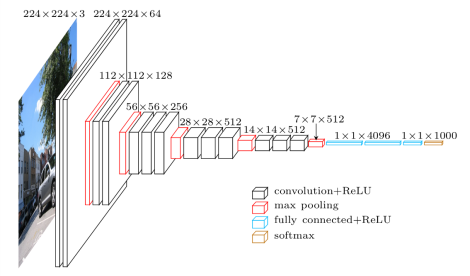
\includegraphics[scale=0.6]{imagenet_vgg16.png}
	\caption{VGG16 on ImageNet}
	\cite{simonyan2014very}
	\label{fig:vgg16}
\end{figure}

The design of the VGG16 had in mind the ImageNet dataset, where there are 1.000 different classes. The two last fully connected layers of the state of the art model are comprised of 4096 neurons each, leading to much higher parameters complexity. As the dataset used in this work has only 10 classes, the two FC-4096 layers were replaced by one single layer with 512 neurons and RELU activations. This change helped to reduce overfitting when training the network. In addition, the total number of convolutions blocks and pooling was reduced to 3, with the first layer having 2 stacked convolution layers followed by a max pooling of stride 2x2 and the last two layers with 3 stacked convolutions also followed by a max pooling of stride 2x2. The max pooling layers are responsible for reducing the image size by 50\% every time an image passes through it. Since CIFAR-10 images are only 32x32, the original VGG16 architecture would end up having an output of shape of only 1x1 pixels at the last layer. In order to avoid this problem, the number of layers were reduced so to fit our dataset domain. The resulting shape fed into the fully connected layers is 4x4x128 (Width x Height x Channels) as it can be seen on table ~\ref{tbl:vgg10}. 

\begin{table}[!h]
	\centering
	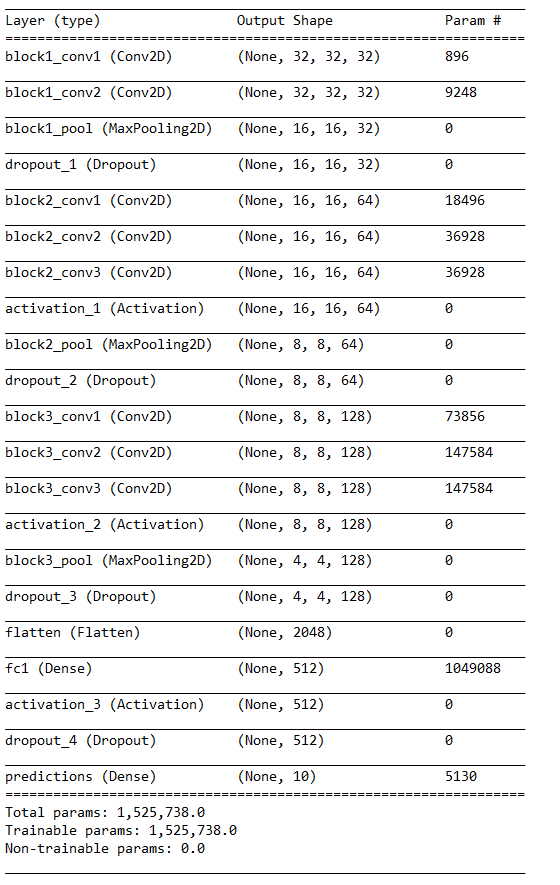
\includegraphics[scale=0.9]{vgg_arch.png}
	\caption{Full Model Description}
	\label{tbl:vgg10}
\end{table}
 
\section{Training Process}

Neural Networks progress was stuck for so many years due to the lack of computational power and good optimisation methods required to extract good performance from these methods. As networks get deeper, the number of resources required to train increases considerably. Even that the Convolutional Neural networks used in the work can share parameters within its convolution layers, we still need to use efficient gradient methods to be able to converge in a reasonable time. All the models comprised in this work were implemented using Python programming language along with Tensorflow and Keras frameworks. The first is a high performance calculation engine that uses GPUs to accelerate its matrix/vector calculations. The latter is a Neural Network library that helps on the implementation of any deep learning model. Keras is mainly a wrapper on top of tensorflow that hides some abstraction from the developer, making it one of the best frameworks for DNNs currently.

As discussed on Chapter 2, it is not feasible to only update the gradients of the network after one full iteration over the entire dataset. Stochastic Gradient methods were one of the first methods developed to overcome this problem and are still being further developed nowadays. The SGD based optimisation technique used in this work was developed by Bengio (2015) \cite{bengiormsprop}, namely RMSProp. This method is an adaptive learning rate scheme that can take the absolute values of the Hessian's eigenvalues and, therefore, approximate the equilibration preconditioner. As shown on Bengio's work \cite{bengiormsprop}, the method outperforms current SGD methods by achieving convergence faster.The learning rate for the method was set at $10^{-4}$ and the decay $10^{-5}$.

In order to achieve good performance, every algorithm should be trained until it converges. Avoiding overfitting and underfitting is highly important when training DNNs. Our architecture was trained until no more reasonable changes were detected in the validation loss so we could dismiss unnecessary training steps and consequently any kind of overfitting. This was achieved by using the Early Stopping technique as described on \cite{stanford2016}. Fundamentally, this consists of a functional callback that runs at the end of every epoch and compares the previous loss with the current one and interrupts training if the difference was below a user provided $\delta$ for a specific number of steps in a row. The value of our $\delta$ was set at $10^{-4}$ and the number of steps to 10. For instance, training would be stopped if no improvement over the specified $\delta$ was seen for 10 steps in a row. Also, we did put a hard limit of 200 on the total number of epochs.

\begin{figure}[!h]
	\centering
	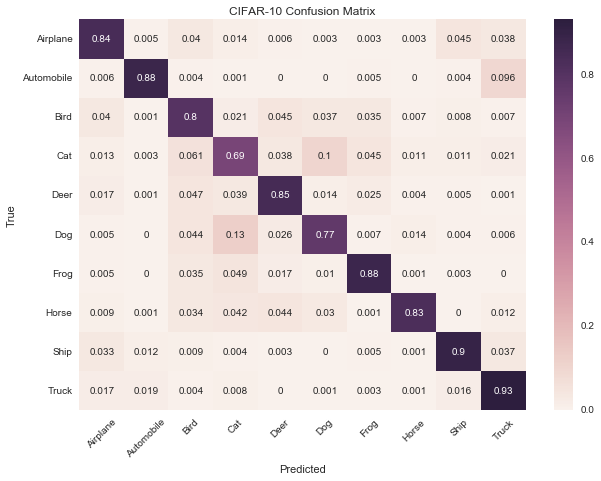
\includegraphics[scale=0.6]{conf_matrix.png}
	\caption{Results on the full dataset}
	\label{fig:conf_matrix}
\end{figure}

The confusion matrix helps understanding the individual score for each class and also which targets class were being missclassified into. Figure ~\ref{fig:conf_matrix} shows that the Cat and Dog classes are often interchangeably missclassified as they have a set of similar features. The network have reached an overall accuracy of 83.45\% and a total validation loss of 0.5033.


\section{Class Imbalanced Training}

Classification models are usually required to have similar number of samples of each class so it could equally learn feature representations for each label. As shown on Murphey and Guo (2004) \cite{murphey2004}, Neural Networks have lower generalization capabilities and are biased towards specific classes when trained on datasets with big number of samples differences between classes. Since our dataset of choice is not an imbalanced case, we randomly removed 4000 samples from each class at a time, creating 10 different datasets.


For each of the 10 different class imbalance dataset configuration, a network was trained until convergence using the same parameters as it was aforementioned. Each model was evaluated against a test set of 1000 equally distributed samples and the results are shown on table ~\ref{tbl:unbl_results}. These models will be the starting point for evaluating adversarial robustness later. The initial performance evaluation of each dataset was based on the Overall Accuracy, validation loss and class specific accuracy. Results are shown on table ~\ref{tbl:unbl_results}.


\begin{table}[!h]
	\begin{tabular}{|c|c|c|c|c|}
		\hline 
		 \multicolumn{1}{|p{2cm}|}{\centering Class \\ Label} & 
		 \multicolumn{1}{|p{3cm}|}{\centering Overall \\ Accuracy}& 
		 \multicolumn{1}{|p{3cm}|}{\centering Validation \\ Loss}& 
		 \multicolumn{1}{|p{3cm}|}{\centering Class-Specific \\ Accuracy}& 
		 Delta (\%) \\ 
		\hline 
		Airplane  & 80.26\%  & 0.5731 & 69\% & 15\%  \\ 
		\hline 
		Automobile & 81.85\%  & 0.5424 & 77\% & 11\%  \\ 
		\hline 
		Bird & 80.75\%  & 0.5797 & 48\% & 32\% \\ 
		\hline 
		Cat & 79.31\%  & 0.5966 & 26\% & 43\%  \\ 
		\hline 
		Deer & 81.36\%  & 0.5497 & 70\% & 15\% \\ 
		\hline 
		Dog & 81.96\% & 0.5525 & 58\% & 17\% \\ 
		\hline 
		Frog & 83.38\%  & 0.5071 & 83\% & 5\% \\ 
		\hline 
		Horse & 82.39\%  & 0.531 & 69\% & 14\% \\ 
		\hline 
		Ship & 83.33\%  & 0.5133 & 80\% & 10\%\\ 
		\hline 
		Truck & 83.48\%  & 0.5215 & 80\% & 13\%\\ 
		\hline 
	\end{tabular} 
	\caption{CNN Imbalanced Dataset Performance. The delta is calculated from the balanced network results on Figure ~\ref{fig:conf_matrix}}
	\label{tbl:unbl_results}
\end{table}


